\chapter{内核、Boot和printf}

\section{实验目的}
  \begin{enumerate}
    \item 从操作系统角度理解MIPS体系结构
    \item 掌握操作系统启动的基本流程
    \item 掌握ELF文件的结构和功能
  \end{enumerate}
在本章中,我们需要阅读并填写部分代码,使得我们的小操作系统可以正常的运行起来。这一章节的难度较为简单。
    
\section{操作系统的启动}

\subsection{内核在哪里?}
通过《计算机组成原理》课的学习,我们知道计算机是由硬件和软件组成的,仅有一个裸机是什么也干不了的;
另一方面,软件也必须运行在硬件之上才能实现其价值。由此可见,硬件和软件是相互依存、密不可分的。
为了能较好的管理计算机系统的硬件资源,我们需要使用操作系统。
那么在操作系统设计课程中,我们管理的硬件在哪里呢?如果足够细心的话,在前面的内容学习可以知道GXemul是一款计算机架构仿真器,在本实验可以模拟我们需要的硬件环境,也就是说我们在《计算机组成原理》课程中辛辛苦苦搭建的CPU等硬件环境,在操作系统实验中已经由GXemul准备好了。在编写操作系统之前,我们每个人面前都是一个裸机。对于操作系统课程设计,我们编写代码的平台是Linux系统,进行仿真实验的平台是GXemul。我们编写的所有的代码,在提供的 Linux平台通过 Makefile 交叉编译产生可执行文件,最后使用GXemul对可执行文件运行填充完成的操作系统。

\begin{note}
操作系统的启动英文称作“boot”。这个词是bootstrap的缩写,意思是鞋带(靴子上的那种)。
之所以将操作系统启动称为boot,源自于一个英文的成语“pull oneself up by one's bootstraps”,
直译过来就是用自己的鞋带把自己提起来。操作系统启动的过程正是这样一个极度纠结的过程。
硬件是在软件的控制下执行的,而当刚上电的时候,存储设备上的软件又需要由硬件载入到内存中去执行。
可是没有软件的控制,谁来指挥硬件去载入软件?因此,就产生了一个类似于鸡生蛋,蛋生鸡一样的问题。
硬件需要软件控制,软件又依赖硬件载入。就好像要用自己的鞋带把自己提起来一样。
早期的工程师们在这一问题上消耗了大量的精力。所以,他们后来将“启动”这一纠结的过程称为“boot”。
\end{note}

操作系统最重要的部分是操作系统内核,因为内核需要直接与硬件交互管理各个硬件,从而利用硬件的功能为用户进程提供服务。
启动操作系统,我们就需要将内核代码在计算机结构上运行起来,一个程序要能够运行,其代码必须能够被CPU直接访问,所以不能在磁盘上,因为CPU无法直接访问磁盘;
另一方面,内存RAM是易失性存储器,掉电后将丢失全部数据,所以不可能将内核代码保存在内存中。
所以直观上可以认识到:①磁盘不能直接访问②内存掉电易失,内核文件有可能放置的位置只能是CPU能够直接访问的非易失性存储器——ROM或FLASH中。

但是,把操作系统内核放置在这种非易失存储器上会有一些问题:
\begin{enumerate}
  \item 这种CPU能直接访问的非易失性存储器的存储空间一般会映射到CPU寻址空间的某个区域,这个是在硬件设计上决定的。
显然这个区域的大小是有限的,如果功能比较简单的操作系统还能够放在其中,对于内核文件较大的普通操作系统而言显然是不足够的。
  \item 如果操作系统内核在CPU加电后直接启动,意味着一个计算机硬件上只能启动一个操作系统,这样的限制显然不是我们所希望的。
  \item 把特定硬件相关的代码全部放在操作系统中也不利于操作系统的移植工作。
\end{enumerate}

基于上述考虑,设计人员一般都会将硬件初始化的相关工作放在名为“bootloader”的程序中来完成。这样做的好处正对应上述的问题:
\begin{enumerate}
  \item 将硬件初始化的相关工作从操作系统中抽出放在bootloader中实现,意味着通过这种方式实现了硬件启动和软件启动的分离。
因此需要存储在非易失性存储器中的硬件启动相关指令不需要很多,能够很容易地保存在ROM或FLASH中。
  \item bootloader在硬件初始化完后,需要为软件启动(即操作系统内核的功能)做相应的准备,
比如需要将内核镜像文件从存放它的存储器(比如磁盘)中读到RAM中。既然bootloader需要将内核镜像文件加载到内存中,
那么它就能选择使用哪一个内核镜像进行加载,即实现多重开机的功能。使用bootloader后,我们就能够在一个硬件上运行多个操作系统了。
  \item bootloader主要负责硬件启动相关工作,同时操作系统内核则能够专注于软件启动以及对用户提供服务的工作,
从而降低了硬件相关代码和软件相关代码的耦合度,有助于操作系统的移植。需要注意的是这样做并不意味着操作系统不依赖硬件。
由于操作系统直接管理着计算机所有的硬件资源,要想操作系统完全独立于处理器架构和硬件平台显然是不切实际的。
然而使用bootloader更清晰地划分了硬件启动和软件启动的边界,使操作系统与硬件交互的抽象层次提高了,从而简化了操作系统的开发和移植工作。
\end{enumerate}

\subsection{Bootloader}
从操作系统的角度看,boot loader 的总目标就是正确地调用内核来执行。
另外,由于 boot loader 的实现依赖于 cpu 的体系结构,因此大多数boot loader 都分为 stage1 和 stage2两大部分。

在stage 1时,此时需要初始化硬件设备,包括watchdog timer、中断、时钟、内存等。需要注意的一个细节是,此时内存RAM尚未初始化完成,
因而stage 1直接运行在存放bootloader的存储设备上(比如FLASH)。由于当前阶段不能在内存RAM中运行,其自身运行会受诸多限制,
比如有些flash程序不可写,即使程序可写的flash也有存储空间限制。这就是为什么需要stage 2的原因。
stage 1除了初始化基本的硬件设备以外,会为加载stage 2准备RAM空间,然后将stage 2的代码复制到RAM空间,并且设置堆栈,最后跳转到stage 2的入口函数。

stage 2运行在RAM中,此时有足够的运行环境从而可以用C语言来实现较为复杂的功能。
这一阶段的工作包括,初始化这一阶段需要使用的硬件设备以及其他功能,然后将内核镜像文件从存储器读到RAM中,并为内核设置启动参数,
最后将CPU指令寄存器的内容设置为内核入口函数的地址,即可将控制权从bootloader转交给操作系统内核。

从CPU上电到操作系统内核被加载的整个启动的步骤如图\ref{fig:bootloader-steps}所示。

\begin{figure}[htbp]
  \centering
  \includegraphics[width=10cm]{bootloader-steps}
  \caption{启动的基本步骤}\label{fig:bootloader-steps} 
\end{figure}

需要注意的是,以上bootloader的两个工作阶段只是从功能上论述内核加载的过程,在具体实现上不同的系统可能有所差别,而且对于不同的硬件环境也会有些不同。
在我们常见的x86 PC的启动过程中,首先执行的是BIOS中的代码,主要完成硬件初始化相关的工作,
然后BIOS会从MBR(master boot record,开机硬盘的第一个扇区)中读取开机信息。在Linux中常说的Grub和Lilo这两种开机管理程序就是保存在MBR中。

\begin{note}
GRUB(GRand Unified Bootloader)是GNU项目的一个多操作系统启动程序。简单的说,就是可以可以用于在有多个操作系统的机器上,
在刚开机的时候选择一个操作系统进行引导。如果安装过Ubuntu一类的发行版的话, 一开机出现的那个选择系统用的菜单就是GRUB提供的。
\end{note}

(这里以Grub为例)BIOS加载MBR中的Grub代码后就把CPU交给了Grub,Grub的工作就是一步一步的加载自身代码,从而识别文件系统,
然后就能够将文件系统中的内核镜像文件加载到内存中,并将CPU控制权转交给操作系统内核。
这样看来,其实BIOS和Grub的前一部分构成了前述stage 1的工作,而stage 2的工作则是完全在Grub中完成的。

\begin{note}
bootloader有两种操作模式:启动加载模式和下载模式。对于普通用户而言,bootloader只运行在启动加载模式,就是我们之前讲解的过程。
而下载模式仅仅对于开发人员有意义,区别是前者是通过本地设备中的内核镜像文件启动操作系统的,而后者是通过串口或以太网等通信手段将远端的内核镜像上载到内存的。
\end{note}

\subsection{gxemul中的启动流程}
从前面的分析,我们可以看到,操作系统的启动是一个非常复杂的过程。不过,幸运的是,由于我们的小操作系统的目标是在gxemul仿真器上运行,
这个过程被大大简化了。gxemul仿真器支持直接加载elf格式的内核,也就是说,gxemul已经提供了bootloader全部功能。
我们的小操作系统不需要再实现bootloader的功能了。换句话说,你可以假定,从我们的小操作系统的运行第一行代码前,
我们就已经拥有一个正常的C环境了。全局变量、函数调用等等C语言运行所需的功能已经可以正常使用了。

\begin{note}
如果你以前对于操作系统的概念仅仅停留在很表面的层次上,那么这里你也许会有所疑惑,为什么我们这里要说“正常的C环境”?
难道还能有“不正常的C环境”?我们来举一个例子说明一下:假定我们刚加电,CPU开始从ROM上取指。
为了简化,我们假定这台机器上没有BIOS(Basic Input Output System),bootloader被直接烧在了ROM中(很多嵌入式环境就是这样做的)。
这时,由于内存没有被初始化,整个bootloader程序尚处于ROM中。程序中的全局变量也仍被储存在ROM上。
而ROM是只读的,所以任何对于全局变量的赋值操作都是不被允许的。可见,此时我们尚不能正常使用C语言的一些特性。
而当内存被初始化,bootloader将后续代码载入到内存中后,位于内存中的代码便能完整地使用C语言的各类功能了。
所以说,内存中的代码拥有了一个正常的C环境。
\end{note}

gxemul支持加载elf格式内核,所以启动流程被简化为加载内核到内存,之后跳转到内核的入口。启动完毕:)整个启动过程非常简单。
这里要注意,之所以简单还有一个原因就在于gxemul本身是仿真器,是一种软件而不是真正的硬件,
所以就不需要面对传统的bootloader面对的那种非常纠结的情况了。

\section{Let's hack the kernel!}

接下来,我们就要开始来折腾我们的小操作系统内核了。这一节中,我们将介绍如何修改内核并实现一些自定义的功能。

\subsection{Makefile——内核代码的地图}
我们来看一下我们的小操作系统的最顶层的Makefile。由于Makefile是用于指导程序如何被构建的,
因此,通过阅读Makefile,我们就可以理解源代码被构建成可执行文件的过程。这一过程可以给我们一些阅读代码的提示,
可以说,Makefile就像源代码的地图,告诉你源代码是如何一步一步成为最终的可执行文件的。代码\ref{code:top-makefile}是实验代码最顶层的Makefile,
通过阅读它我们就能了解代码中很多宏观的东西。

\begin{codeBoxWithCaption}{顶层Makefile\label{code:top-makefile}}
  \inputminted[linenos]{make}{codes/top-Makefile}
\end{codeBoxWithCaption}

如果你以前没有接触过Makefile的话,突然看到这份40行的Makefile可能会有些无奈,完全看不懂啊。不必着急,我们来一行一行地解读它。
前6行是注释,你懂得。7~21行定义了一些变量,包括各个子目录的相对路径,最终的可执行文件的路径(vmlinux\_elf),
linker script的位置(link\_script)。值得注意的两个是modules定义了内核所包含的所有模块,而objects则表示要编译出内核所依赖的所有.o文件。
17到21行行末的斜杠代表这一行没有结束,下一行的内容和这一行是连在一起的。这种写法一般用于提高文件的可读性。可以把本该写在同一行的东西分布在多行中,
使得文件更容易被人类阅读。

\begin{note}
linker script是用于指导连接器将多个.o文件连接成目标可执行文件的脚本。.o文件、linker script等内容我们会在下面的小节中细致地讲解,
大家这里只要知道这些文件是编译内核所必要的就好。
\end{note}

23行的.PHONY表明列在其后的规则不受修改时间的约束。也就是说,一旦该规则被调用,一定保证它被执行。第25行定义all这一规则的依赖。
all代表整个项目,由此我们可以知道,构建整个项目依赖于构建好所有的模块以及vmlinux。那么vmlinux是如何被构建的呢?
紧接着的27行定义了,vmlinux的构建依赖于所有的模块。在构建完所有模块后,将执行第28行的指令来产生vmlinux。
我们可以看到,第28行调用了连接器将之前构建各模块产生的所有.o文件在linker script的指导下连接到一起,产生最终的vmlinux可执行文件。
第30行定义了每个模块的构建方法为调用对应模块目录下的Makefile。最后的33到38行定义了如何清理所有被构建出来的文件。

\begin{note}
一般在写Makefile时,习惯将第一个规则命名为all,也就是构建整个项目的意思。如果调用make时没有指定目标,make会自动执行第一个目标,
所以把all放在第一个目标的位置上,可以使得make命令默认构建整个项目,较为方便。
\end{note}

读到这里,我们会发现还有几个关键的变量没有定义。是的,就是LD、MAKE等出现在编译指令中的变量。紧接着我们看到了第40行有一条include命令。
看来,这个顶层的Makefile还引用了其他的东西。显然这些未定义的变量,是被定义在了这个被include的文件中。被引用的文件如代码\ref{code:include-mk}所示。

\begin{codeBoxWithCaption}{include.mk\label{code:include-mk}}
  \inputminted[linenos]{make}{codes/include.mk}
\end{codeBoxWithCaption}

在该文件中,我们看到了一个非常熟悉的关键词——Cross Compile(交叉编译)。不难看出,这里的CROSS\_COMPILE变量是在定义编译和连接等指令的前缀,
或者说是交叉编译器的具体位置。例如,LD最终调用的指令是“/opt/eldk/usr/bin/mips\_4KC-ld”。通过修改该变量,就可以方便地设定交叉编译工具链的位置。

\begin{exercise}
请修改include.mk文件,使交叉编译器的路径正确。之后执行make指令,如果配置一切正确,则会在gxemul目录下生成vmlinux的内核文件。
\end{exercise}

至此,我们就可以大致掌握阅读Makefile的方法了。善于运用make的功能可以给你带来很多惊喜哦:)提示:可以试着使用一下make clean。
如果你觉得每次用gxemul运行内核都需要打很长的指令这件事很麻烦,那么可以尝试在Makefile中添加运行内核这一功能,使得通过make就能自动运行内核。

\subsection{ELF——深入探究编译与链接}
如果你已经尝试过运行内核,那么你会发现它现在是根本运行不起来的。因为我们还有一些重要的步骤没有做。但是在做这些之前,我们不得不补充一些重要的,
但又有些琐碎的知识。在这里,我们将掀开可执行文件的神秘面纱,进一步去了解一段代码是如何从编译一步一步变成一个可执行文件以及可执行文件又是如何被执行的。

在一切开始之前,请你先泡好一杯茶,慢慢地、耐心地读下去。这一部分的知识对于后面十分重要,但又十分冗长。我们会尽量说得轻松活泼一些,
但由于知识本身的琐碎以及不连贯,所以阅读体验并不会很好。请注意我们在本章中阐述的内容一部分关于Linux实验环境,即在Linux环境下如何模拟我们编写的操作系统,另一部分则是关于我们将要编写的操作系统,在看琐碎的知识点时,请务必注意我们在讨论哪一部分,本章很多概念的混淆或模糊都是由于没有区分开这两部分内容。请务必坚持看完:)

\begin{codeBoxWithCaption}{一个简单的C程序\label{code:hello-c}}
  \inputminted[linenos]{c}{codes/hello.c}
\end{codeBoxWithCaption}

我们以代码\ref{code:hello-c}为例,讲述我们这个冗长的故事。我们首先探究这样一个问题:\textbf{含有多个C文件的工程是如何编译成一个可执行文件的?}

这段代码相信你非常熟悉了,不知你有没有注意到过这样一个小细节:printf的定义在哪里?
\footnote{printf位于标准库中,而不在我们的C代码中。将标准库和我们自己编写的C文件编译成一个可执行文件的过程,与将多个C文件编译成一个可执行文件的过程相仿。
因此,我们通过探究printf如何和我们的C文件编译到一起,来展示整个过程。}
我们都学过,C语言中函数必须有定义才能被调用,那么printf的定义在哪里呢?你一定会笑一笑说,别傻了,不就在stdio.h中吗?我们在程序开头通过include引用了它的。
然而事实真的是这样吗?我们来进去看一看stdio.h里到底有些什么。

\begin{codeBoxWithCaption}{stdio.h中关于printf的内容\label{code:part-stdio-h}}
  \inputminted[linenos]{c}{codes/part_of_stdio.h}
\end{codeBoxWithCaption}

在代码\ref{code:part-stdio-h}中,我们展示了从当前系统的stdio.h中摘录出的与printf相关的部分。可以看到,我们所引用的stdio.h中只有声明,但并没有printf的定义。
或者说,并没有printf的具体实现。可没有具体的实现,我们究竟是如何调用printf的呢?我们怎么能够调用一个没有实现的函数呢?

我们来一步一步探究,printf的实现究竟被放在了哪里,又究竟是在何时被插入到我们的程序中的。首先,我们要求编译器\textbf{只进行预处理(通过-E选项)},而不编译。

\begin{minted}[linenos]{c}
/* 由于原输出太长,这里只能留下很少很少的一部分。 */
typedef unsigned char __u_char;
typedef unsigned short int __u_short;
typedef unsigned int __u_int;
typedef unsigned long int __u_long;


typedef signed char __int8_t;
typedef unsigned char __uint8_t;
typedef signed short int __int16_t;
typedef unsigned short int __uint16_t;
typedef signed int __int32_t;
typedef unsigned int __uint32_t;

typedef signed long int __int64_t;
typedef unsigned long int __uint64_t;

extern struct _IO_FILE *stdin;
extern struct _IO_FILE *stdout;
extern struct _IO_FILE *stderr;

extern int printf (const char *__restrict __format, ...);

int main()
{
    printf("Hello World!\n");
    return 0;
}
\end{minted}

可以看到,C语言的预处理器将头文件的内容添加到了源文件中,但同时我们也能看到,这里一阶段并没有printf这一函数的定义。

之后,我们将gcc的-E选项换为-c选项,\textbf{只编译而不链接},产生一个.o目标文件。
我们对其进行反汇编\footnote{为了便于你重现,我们这里没有选择MIPS,而选择了在流行的x86-64体系结构上进行反汇编。
同时,由于x86-64的汇编是CISC汇编,看起来会更为清晰一些。},结果如下

\begin{minted}[linenos]{objdump}
hello.o:     file format elf64-x86-64

Disassembly of section .text:

0000000000000000 <main>:
   0:   55                      push   %rbp
   1:   48 89 e5                mov    %rsp,%rbp
   4:   bf 00 00 00 00          mov    $0x0,%edi
   9:   e8 00 00 00 00          callq  e <main+0xe>
   e:   b8 00 00 00 00          mov    $0x0,%eax
  13:   5d                      pop    %rbp
  14:   c3                      retq
\end{minted}

我们只需要注意中间那句callq即可,这一句是调用函数的指令。对照左侧的机器码,其中e8是call指令的操作码。根据我们在《计算机组成》课程中学习MIPS跳转指令的经验,
e8后面应该跟的是printf的地址。可在这里我们却发现,\textbf{本该填写printf地址的位置上被填写了一串0}。那个地址显然不可能是printf的地址。也就是说,直到这一步,
printf的具体实现依然不在我们的程序中。

最后,我们允许gcc进行连接,也就是\textbf{正常地编译}出可执行文件。然后,再用objdump进行反汇编。

\begin{minted}[linenos]{objdump}
hello:     file format elf64-x86-64


Disassembly of section .init:

00000000004003a8 <_init>:
  4003a8:       48 83 ec 08             sub    $0x8,%rsp
  4003ac:       48 8b 05 0d 05 20 00    mov    0x20050d(%rip),%rax
  4003b3:       48 85 c0                test   %rax,%rax
  4003b6:       74 05                   je     4003bd <_init+0x15>
  4003b8:       e8 43 00 00 00          callq  400400 <__gmon_start__@plt>
  4003bd:       48 83 c4 08             add    $0x8,%rsp
  4003c1:       c3                      retq   

Disassembly of section .plt:

00000000004003d0 <puts@plt-0x10>:
  4003d0:       ff 35 fa 04 20 00       pushq  0x2004fa(%rip)
  4003d6:       ff 25 fc 04 20 00       jmpq   *0x2004fc(%rip)
  4003dc:       0f 1f 40 00             nopl   0x0(%rax)

00000000004003e0 <puts@plt>:
  4003e0:       ff 25 fa 04 20 00       jmpq   *0x2004fa(%rip)
  4003e6:       68 00 00 00 00          pushq  $0x0
  4003eb:       e9 e0 ff ff ff          jmpq   4003d0 <_init+0x28>

00000000004003f0 <__libc_start_main@plt>:
  4003f0:       ff 25 f2 04 20 00       jmpq   *0x2004f2(%rip)
  4003f6:       68 01 00 00 00          pushq  $0x1
  4003fb:       e9 d0 ff ff ff          jmpq   4003d0 <_init+0x28>

0000000000400400 <__gmon_start__@plt>:
  400400:       ff 25 ea 04 20 00       jmpq   *0x2004ea(%rip)
  400406:       68 02 00 00 00          pushq  $0x2
  40040b:       e9 c0 ff ff ff          jmpq   4003d0 <_init+0x28>

Disassembly of section .text:

0000000000400410 <main>:
  400410:       48 83 ec 08             sub    $0x8,%rsp
  400414:       bf a4 05 40 00          mov    $0x4005a4,%edi
  400419:       e8 c2 ff ff ff          callq  4003e0 <puts@plt>
  40041e:       31 c0                   xor    %eax,%eax
  400420:       48 83 c4 08             add    $0x8,%rsp
  400424:       c3                      retq   

0000000000400425 <_start>:
  400425:       31 ed                   xor    %ebp,%ebp
  400427:       49 89 d1                mov    %rdx,%r9
  40042a:       5e                      pop    %rsi
  40042b:       48 89 e2                mov    %rsp,%rdx
  40042e:       48 83 e4 f0             and    $0xfffffffffffffff0,%rsp
  400432:       50                      push   %rax
  400433:       54                      push   %rsp
  400434:       49 c7 c0 90 05 40 00    mov    $0x400590,%r8
  40043b:       48 c7 c1 20 05 40 00    mov    $0x400520,%rcx
  400442:       48 c7 c7 10 04 40 00    mov    $0x400410,%rdi
  400449:       e8 a2 ff ff ff          callq  4003f0 <__libc_start_main@plt>
  40044e:       f4                      hlt    
  40044f:       90                      nop
\end{minted}

篇幅所限,余下的部分没法再展示了(大约还有100来行)。当你看到这段代码的时候,心头一定有一大群草泥马呼啸而过。
什么鬼!我们原本那只可爱的Hello World怎么变成了这副鬼样子!

别急,我们还是只把注意力放在主函数中,这一次,我们可以看到,主函数里那一句callq后面已经不再是一串0了。
那里已经\textbf{被填入了一个地址}。从反汇编代码中我们也可以看到,这个地址就在这个可执行文件里,就在被标记为puts@plt的那个位置上。
虽然高不清楚那货是什么,但显然那就是我们所调用的printf的具体实现了。

由此,我们不难推断,printf的实现是在\textbf{连接(Link)}这一步骤中被插入到最终的可执行文件中的。那么,了解这个细节究竟有什么用呢?
作为一个库函数,printf被大量的程序所使用。因此,每次都将其编译一遍实在太浪费时间了。printf的实现其实早就被编译成了二进制形式。
但此时,printf并未连接到程序中,它的状态与我们利用-c选项产生的hello.o相仿,都还处于未连接的状态。而在编译的最后,
连接器(Linker)会将所有的目标文件连接在一起,将之前未填写的地址等信息填上,形成最终的可执行文件,这就是连接的过程。

对于拥有多个c文件的工程来说,编译器会首先将所有的c文件以文件为单位,编译成.o文件。最后再将所有的.o文件以及函数库连接在一起,
形成最终的可执行文件。整个过程如图\ref{fig:link}所示。

\begin{figure}[htbp]
  \centering
  \includegraphics[width=8cm]{link}
  \caption{编译、连接的过程}\label{fig:link} 
\end{figure}

接下来,我们提出我们的下一个问题:\textbf{连接器通过哪些信息来连接多个目标文件呢?}答案就在于在目标文件(也就是我们通过-c选项生成的.o文件)。
在目标文件中,记录了代码各个段的具体信息。连接器通过这些信息来将目标文件链接到一起。而ELF(Executable and Linkable Format)正是Unix上常用的一种目标文件格式。
其实,不仅仅是目标文件,可执行文件也是使用ELF格式记录的。这一点通过ELF的全称也可以看出来。

为了帮助你了解ELF文件,下一步我们需要进一步探究它的功能以及格式。

ELF文件是一种对可执行文件、目标文件和库使用的文件格式,跟Windows下的PE文件格式类似。ELF格式是是UNIX系统实验室作为ABI(Application Binary Interface)而开发和发布的,现在早已经是Linux下的标准格式了。我们在之前曾经看见过的.o文件就是ELF所包含的三种文件类型中的一种,称为可重定位(relocatable)文件,其它两种文件类型分别是可执行(executable)文件和共享对象(shared object)文件,这两种文件都需要链接器对可重定位文件进行处理才能生成。

你可以使用file命令来获得文件的类型,如图\ref{fig:lab1-file}所示。

\begin{figure}[htbp]
  \centering
  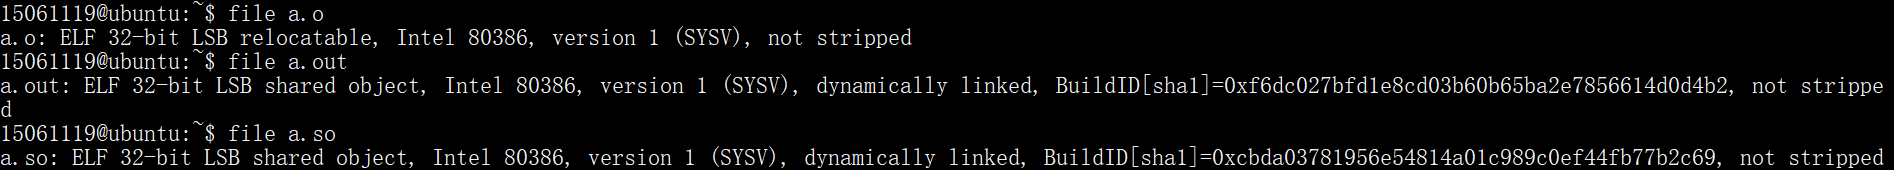
\includegraphics[width=16cm,height=2cm]{lab1-file}
  \caption{file命令}\label{fig:lab1-file} 
\end{figure}

那么,ELF文件中都包含有什么东西呢?简而言之,就是和程序相关的所有必要信息,下图\ref{fig:lab1-elf-1}说明了ELF文件的结构:

\begin{figure}[htbp]
  \centering
  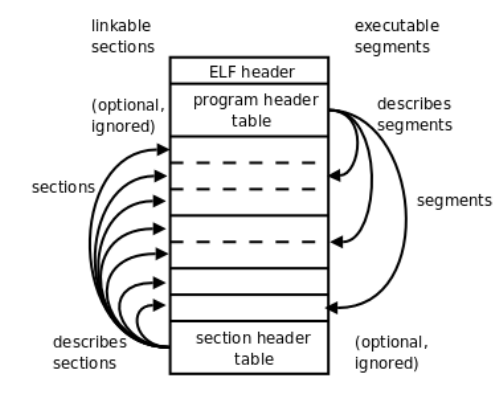
\includegraphics[width=8cm]{lab1-elf-1}
  \caption{ELF文件结构}\label{fig:lab1-elf-1}
\end{figure}

通过上图我们可以知道,ELF文件从整体来说包含5个部分:

\begin{enumerate}
  \item ELF Header,包括程序的基本信息,比如体系结构和操作系统,同时也包含了Section Header Table和Program Header Table相对文件的偏移量(offset)。
  \item Program Header Table,也可以称为Segment Table,主要包含程序中各个Segment的信息,Segment的信息需要在运行时刻使用。
  \item Section Header Table,主要包含各个Section的信息,Section的信息需要在程序编译和链接的时候使用。
  \item Segments,就是各个Segment。Segment则记录了每一段数据(包括代码等内容)需要被载入到哪里,记录了用于指导应用程序加载的各类信息。
  \item Sections,就是各个Section。Section记录了程序的代码段、数据段等各个段的内容,主要是连接器在连接的过程中需要使用。
\end{enumerate}

观察上图\ref{fig:lab1-elf-1}我们可以发现,Program Header Table和Section Header Table指向了同样的地方,这就说明两者所代表的内容是重合的,这意味着什么呢?意味着两者只是同一个东西的不同视图!产生这种情况的原因在于ELF文件需要在两种场合使用:

  \begin{enumerate}
    \item 组成可重定位文件,参与可执行文件和可共享文件的链接。
    \item 组成可执行文件或者可共享文件,在运行时为加载器提供信息。
  \end{enumerate}

我们已经了解了ELF文件的大体结构,现在,我们需要你自己动手,阅读一个简易的对32bitELF文件(little endian)的解析程序,然后完成部分代码,来了解ELF文件各个部分的详细结构。

为了简化你的理解过程,我们先对这个程序中涉及的三个关键数据结构做一下简要说明,请你仔细阅读下面的代码和注释,然后完成练习。
下面的代码都截取自./readelf/kerelf.h文件

\begin{minted}[linenos]{c}

typedef struct
{
  // some identification informtion, including magic number
  unsigned char e_ident[EI_NIDENT];
  // file type, including relocatable file, executable file and shared object
  Elf32_Half e_type;
  // architecture, like MIPS
  Elf32_Half e_machine;
  // version info
  Elf32_Word e_version;
  // addr of entry point
  Elf32_Addr e_entry;
  // program header table offset
  Elf32_Off  e_phoff;
  // section header table offset
  Elf32_Off  e_shoff;
  // relating to processor
  Elf32_Half e_flags;
  // elf header size
  Elf32_Half e_ehsize;
  // program header entry size
  Elf32_Half e_phentsize;
  // program header entry number
  Elf32_Half e_phnum;
  // section header entry size
  Elf32_Half e_shentsize;
  // section header entry number
  Elf32_Half e_shnum;
}Elf32_Ehdr;

typedef struct
{
  // section name
  Elf32_Word sh_name;
  // section type
  Elf32_Word sh_type;
  // section flags
  Elf32_Word sh_flags;
  // section addr
  Elf32_Addr sh_addr;
  // offset from elf head of this entry
  Elf32_Off  sh_offset;
  // byte size of this section
  Elf32_Word sh_size;
  // link
  Elf32_Word sh_link;
  // extra info
  Elf32_Word sh_info;
  // alignment
  Elf32_Word sh_addralign;
  // entry size
  Elf32_Word sh_entsize;
}Elf32_Shdr;

typedef struct
{
  // segment type
  Elf32_Word p_type;
  // offset from elf file head of this entry
  Elf32_Off  p_offset;
  // virtual addr of this segment
  Elf32_Addr p_vaddr;
  // physical addr, in linux, this value is meanless and has same value of p_vaddr
  Elf32_Addr p_paddr;
  // file size of this segment
  Elf32_Word p_filesz;
  // memory size of this segment
  Elf32_Word p_memsz;
  // segment flag
  Elf32_Word p_flags;
  // alignment
  Elf32_Word p_align;
}Elf32_Phdr;
\end{minted}

\begin{exercise}
阅读./readelf文件夹中kerelf.h、readelf.c以及main.c三个文件中的代码,并完成readelf.c中缺少的代码,readelf函数需要输出elf文件的所有section header的序号和地址信息,对每个section header,输出格式为:"\%d:0x\%x$\backslash$n",两个标识符分别代表序号和地址。
\end{exercise}

\begin{thinking}\label{think-endian}
也许你会发现我们的readelf程序是不能解析之前生成的内核文件(内核文件是可执行文件)的,而我们之后将要介绍的工具readelf则可以解析,这是为什么呢?(提示:尝试使用readelf -h,观察不同)
\end{thinking}

通过刚才的练习,相信你已经对ELF文件有了一个比较充分的了解,你可能想进一步解析ELF文件来获得更多的信息,不过这个工作已经有人帮你做了,使用readelf工具,你就可以很方便地解析ELF文件。
现在,我们继续内核的话题。

我们最终生成的内核也是ELF格式的,被模拟器载入到内核中。因此,我们暂且只关注ELF是如何被载入到内核中,并且被执行的,
而不再关心具体的连接细节。也即上文旨在探索关于我们实验环境的编译连接问题。在阅读完上面编译和ELF的说明后,应该明确我们OS实验课如何编译连接产生实验操作系统的可执行文件并且gxemul运行模拟该ELF文件。ELF中有两个相似却不同的概念segment和section,我们之前已经提到过。

我们不妨来看一下,我们之前那个hello world程序的各个segment长什么样子。readelf工具可以方便地解析出elf文件的内容,这里我们使用它来分析我们的程序。
首先我们使用-l参数来查看各个segment的信息。

\begin{minted}[linenos]{objdump}
Elf 文件类型为 EXEC (可执行文件)
入口点 0x400e6e
共有 5 个程序头,开始于偏移量64

程序头:
  Type           Offset             VirtAddr           PhysAddr
                 FileSiz            MemSiz              Flags  Align
  LOAD           0x0000000000000000 0x0000000000400000 0x0000000000400000
                 0x00000000000b33c0 0x00000000000b33c0  R E    200000
  LOAD           0x00000000000b4000 0x00000000006b4000 0x00000000006b4000
                 0x0000000000001cd0 0x0000000000003f48  RW     200000
  NOTE           0x0000000000000158 0x0000000000400158 0x0000000000400158
                 0x0000000000000044 0x0000000000000044  R      4
  TLS            0x00000000000b4000 0x00000000006b4000 0x00000000006b4000
                 0x0000000000000020 0x0000000000000050  R      8
  GNU_STACK      0x0000000000000000 0x0000000000000000 0x0000000000000000
                 0x0000000000000000 0x0000000000000000  RW     10

 Section to Segment mapping:
  段节...
   00     .note.ABI-tag .note.gnu.build-id .rela.plt .init .plt .text 
   __libc_freeres_fn __libc_thread_freeres_fn .fini .rodata __libc_subfreeres 
   __libc_atexit __libc_thread_subfreeres .eh_frame .gcc_except_table 
   01     .tdata .init_array .fini_array .jcr .data.rel.ro .got .got.plt .data 
   .bss __libc_freeres_ptrs 
   02     .note.ABI-tag .note.gnu.build-id 
   03     .tdata .tbss 
   04
\end{minted}

这些输出中,我们只需要关注这样几个部分:Offset代表该段(segment)的数据相对于ELF文件的偏移。VirtAddr代表该段最终需要被加载到内存的哪个位置。
FileSiz代表该段的数据在文件中的长度。MemSiz代表该段的数据在内存中所应当占的大小。

\begin{note}
MemSiz永远大于等于FileSiz。若MemSiz大于FileSiz,则操作系统在加载程序的时候,会首先将文件中记录的数据加载到对应的VirtAddr处。
之后,向内存中填0,直到该段在内存中的大小达到MemSiz为止。那么为什么MemSiz有时候会大于FileSiz呢?这里举这样一个例子:
C语言中未初始化的全局变量,我们需要为其分配内存,但它又不需要被初始化成特定数据。因此,在可执行文件中也只记录它需要占用内存(MemSiz),
但在文件中却没有相应的数据(因为它并不需要初始化成特定数据)。故而在这种情况下,MemSiz会大于FileSiz。这也解释了,
为什么C语言中全局变量会有默认值0。这是因为操作系统在加载时将所有未初始化的全局变量所占的内存统一填了0。
\end{note}

VirtAddr是我们尤为需要注意的。由于它的存在,我们就不难推测,Gxemul仿真器在加载我们的内核时,是按照内核这一可执行文件中所记录的地址,
将我们内核中的代码、数据等加载到相应位置。并将CPU的控制权交给内核。我们的内核之所以不能够正常运行,显然是因为我们内核所处的地址是不正确的。
换句话说,\textbf{只要我们能够将内核加载到正确的位置上,我们的内核就应该可以运行起来。}

思考到这里,我们又发现了几个重要的问题。
\begin{enumerate}
  \item 当我们讲加载操作系统内核到正确的Gxemul模拟物理地址时,讨论的是Linux实验环境呢?还是我们编写的操作系统本身呢?
  \item 什么叫做正确的位置?到底放在哪里才叫正确。
  \item 哪个段被加载到哪里是记录在编译器编译出来的ELF文件里的,我们怎么才能修改它呢?
\end{enumerate}
在接下来的小节中,我们将一点一点解决掉这两个问题。

\subsection{MIPS内存布局——寻找内核的正确位置}
在这一节中,我们来解决关于内核应该被放在何处的问题。在32位的MIPS CPU中,程序地址空间会被划分为4个大区域。如图\ref{fig:memory-region}所示。

\begin{figure}[htbp]
  \centering
  \includegraphics[height=8cm]{memory-region}
  \caption{MIPS内存布局}\label{fig:memory-region} 
\end{figure}

从硬件角度讲,这四个区域的情况如下:

\begin{enumerate}
  \item User Space(kuseg) 0x00000000-0x7FFFFFFF(2G):这些是用户模式下可用的地址。在使用这些地址的时候,程序会通过MMU映射到实际的物理地址上。
  \item Kernel Space Unmapped Cached(kseg0) 0x80000000-0x9FFFFFFF(512MB):只需要将地址的高3 位清零,这些地址就被转换为物理地址。
也就是说,逻辑地址到物理地址的映射关系是硬件直接确定,不通过MMU。因为转换很简单,我们常常把这些地址称为“无需转换的”。
一般情况下,都是通过cache 对这段区域的地址进行访问。
  \item Kernel Space Unmapped Uncached(kseg1) 0xA0000000-0xBFFFFFFF(512MB):这一段地址的转换规则与前者相似,
通过将高3 位清零的方法将地址映射为相应的物理地址,然后映射到物理内存中512MB 大小的低字段。需要注意的是,kseg1 不通过cache 进行存取。
  \item Kernel Space Mapped Cached(kseg2) 0xC0000000-0xFFFFFFFF(1GB):这段地址只能在内核态下使用并且需要MMU 的转换。
\end{enumerate}

看到这里,你也许又蔫儿了,还是完全不知道该把内核放在哪里呀!这里,我们再提供一个提示:需要通过MMU映射访问的地址得在建立虚拟内存机制后才能正常使用,
是由操作系统所管理的。因此,在载入内核时,我们只能选用不需要通过MMU的内存空间,因为此时尚未建立虚存机制。好了,满足这一条件的只有kseg0和kseg1了。
而kseg1是不经过cache的,一般用于访问外部设备。所以,我们的内核只能放在seg0了。

那么具体放在哪里呢?这时,我们就需要仔细阅读代码了。在include/mmu.h里有我们的小操作系统内核完整的内存布局图(代码\ref{code:memory-mmu-h}所示),
在之后的实验中,善用它可以带来意料之外的惊喜。

(Tip:在操作系统实验中,填空的代码往往只是核心部分,而对于实验的理解而言需要阅读的代码有很多,而且在阅读的过程中,希望能够梳理出一个脉络和体系,比如某些代码完成了什么功能,代码间依赖关系是什么?OS课程需要填空的代码并不多,希望本课程结束之后,学弟学妹们具有读懂一段较长的工程代码的能力。而课上测试将建立在理解代码的基础上。)

\begin{codeBoxWithCaption}{include/mmu.h中的内存布局图\label{code:memory-mmu-h}}
  \inputminted[linenos]{c}{codes/memory-mmu.h}
\end{codeBoxWithCaption}

相信聪明的你已经发现了内核的正确位置了吧?

\subsection{Linker Script——控制加载地址}
在发现了内核的正确位置后,我们只需要想办法让内核被加载到那里就OK了(把编写的操作系统放到模拟硬件的某个物理位置)。之前在分析ELF文件时我们曾看到过,编译器在生成ELF文件时就已经记录了各段所需要被加载到的位置。
同时,我们也发现,最终的可执行文件实际上是由连接器产生的(它将多个目标文件连接产生最终可执行文件)。因此,我们所需要做的,就是控制连接器的连接过程。

接下来,我们就要引入一个神奇的东西:Linker Script。连接器的设计者们在设计连接器的时候面临这样一个问题:不同平台的ABI(Application Binary Interface)都不一样,
怎样做才能增加连接器的通用性,使得它能为各个不同的平台生成可执行文件呢?于是,就有了Linker Script。Linker Script中记录了各个section应该如何映射到segment,
以及各个segment应该被加载到的位置。下面的指令可以输出默认的连接脚本,你可以在自己的机器上尝试这一条指令:

\begin{minted}[linenos]{bash}
ld --verbose
\end{minted}

这里,我们再补充一下关于ELF文件中section的概念。在链接过程中,目标文件被看成section的集合,并使用section header table来描述各个section的组织。
换句话说,section记录了在连接过程中所需要的必要信息。其中最为重要的三个段为.text、.data、.bss。这三种段的意义是必须要掌握的:

\begin{description}
  \item[.text] 保存可执行文件的操作指令。
  \item[.data] 保存已初始化的全局变量和静态变量。
  \item[.bss] 保存未初始化的全局变量和静态变量。
\end{description}

以上的描述也许会显得比较抽象,这里我们来做一个实验。我们编写一个用于输出代码、全局已初始化变量和全局未初始化变量地址的代码(如代码\ref{code:sections}所示)。
观察其运行结果与ELF文件中记录的.text、.data和.bss段相关信息之间的关系。

\begin{codeBoxWithCaption}{用于输出各section地址的程序\label{code:sections}}
  \inputminted[linenos]{c}{codes/sections.c}
\end{codeBoxWithCaption}

该程序的一个可能的输出如下\footnote{在不同机器上运行,结果也许会有一定的差异}。

\begin{minted}[linenos]{bash}
user@debian ~/Desktop $ ./program 
80D4188
80D60A0
8048AAC
\end{minted}

我们再看看ELF文件中记录的各section的相关信息(为了突出重点,这里只保留我们所关心的section)。

\begin{minted}[linenos]{objdump}
共有 29 个节头,从偏移量 0x9c258 开始:

节头:
  [Nr] Name              Type            Addr     Off    Size   ES Flg Lk Inf Al
  [ 4] .text             PROGBITS        08048140 000140 0620e4 00  AX  0   0 16
  [22] .data             PROGBITS        080d4180 08b180 000f20 00  WA  0   0 32
  [23] .bss              NOBITS          080d50c0 08c0a0 00136c 00  WA  0   0 64
\end{minted}

对比二者,我们就可以清晰的知道,\textbf{.text段包含了可执行文件中的代码},\textbf{.data段包含了需要被初始化的全局变量和静态变量},
而\textbf{.bss段包含了无需初始化的全局变量和静态变量}

接下来,我们通过Linker Script来尝试调整各段的位置。这里,我们选用GNU LD官方帮助文档上的例子
(\url{https://www.sourceware.org/binutils/docs/ld/Simple-Example.html#Simple-Example})
该例子的完整代码如下所示:

\begin{minted}[linenos]{objdump}
SECTIONS
{
   . = 0x10000;
   .text : { *(.text) }
   . = 0x8000000;
   .data : { *(.data) }
   .bss : { *(.bss) }
}
\end{minted}

在第三行的“.”是一个特殊符号,用来做定位计数器,它根据输出段的大小增长。在SECTIONS命令开始的时候,它的值为0。通过设置“.”即可设置接下来的section的其实地址。
“*”是一个通配符,匹配所有的相应的段。例如“.bss:\{*(.bss)\}”表示将所有输入文件中的.bss段(右边的.bss)都放到输出的.bss段(左边的.bss)中。
为了能够编译通过(这个脚本过于简单,难以用于连接真正的程序),我们将原来的实验代码简化如下

\begin{minted}[linenos]{c}
char msg[]="Hello World!\n";
int count;

int main()
{
    return 0;
}
\end{minted}

编译,并查看生产的可执行文件各section的信息。

\begin{minted}[linenos]{objdump}
user@debian ~/Desktop $ gcc -o test test.c -T test.lds -nostdlib -m32
user@debian ~/Desktop $ readelf -S test                              
共有 11 个节头,从偏移量 0x2164 开始:

节头:
  [Nr] Name              Type            Addr     Off    Size   ES Flg Lk Inf Al
  [ 2] .text             PROGBITS        00010024 001024 00000a 00  AX  0   0  1
  [ 5] .data             PROGBITS        08000000 002000 00000e 00  WA  0   0  1
  [ 6] .bss              NOBITS          08000010 00200e 000004 00  WA  0   0  4
\end{minted}

可以看到,在使用了我们自定义的Linker Script以后,生成的程序各个section的位置就被调整到了我们所指定的地址上。
segment是由section组合而成的,section的地址被调整了,那么最终segment的地址也会相应地被调整。
至此,我们就了解了如何通过lds文件控制各段被加载到的位置。

\begin{exercise}
填写tools/scse0\_3.lds中空缺的部分,将内核调整到正确的位置上。
\end{exercise}

再补充一点:关于链接后的程序从何处开始执行。程序执行的第一条指令称为entry point,
我们在linker script中可以通过ENTRY(function name)指令来设置程序入口。linker中程序入口的设置方法有以下五种:
\begin{enumerate}
  \item 使用ld命令时,通过参数“-e”设置
  \item 在linker scirpt中使用ENTRY()指令指定了程序入口
  \item 如果定义start,则start就是程序入口
  \item .text段的第一个字节
  \item 地址0处
\end{enumerate}
在我们的实验中,采用了其中的第二种方式指定了程序入口。

\section{MIPS汇编与C语言}
在这一节中,我们将简单介绍MIPS汇编,以及常见的C语言语法与汇编的对应关系。在操作系统编程中,不可避免地要接触到汇编语言。
我们经常需要从C语言中调用一些汇编语言写成的函数,或者反过来,在汇编中跳转到C函数。为了能够实现这些,
我们需要了解C语言与汇编之间千丝万缕的联系。

我们代码\ref{code:c-example}为例,介绍典型的C语言中的语句对应的汇编代码。

\begin{codeBoxWithCaption}{样例程序\label{code:c-example}}
  \inputminted[linenos]{c}{codes/example.c}
\end{codeBoxWithCaption}

\subsection{循环与判断}
这里你可能会问了,样例代码里只有循环啊!哪里有什么判断语句呀?事实上,由于MIPS汇编中没有循环这样的高级结构,
所有的循环均是采用判断加跳转语句实现的,所以我们将循环语句和判断语句合并在一起进行分析。
我们分析代码的第一步,就是要将循环等高级结构,用\textbf{判断加跳转}的方式替代。
例如,代码\ref{code:c-example}第13-15行的循环语句,其最终的实现可能就如下面的C代码所展示的那样。

\begin{minted}[linenos]{c}
      i = 0;
      goto CHECK;
FOR:  sum += fib(i);
      ++i;
CHECK:if (i < 10) goto FOR;
\end{minted}

将样例程序编译\footnote{为了生成更简单的汇编代码,我们采用了-nostdlib -static -mno-abicalls这三个编译参数},
我们观察其反汇编代码。对照汇编代码和我们刚才所分析出来的C代码。
我们基本就能够看出来其间的对应关系。这里,我们将对应的C代码标记在反汇编代码右侧。

\begin{minted}[linenos]{objdump}
  400158:       sw      zero,16(s8)           #       sum = 0;
  40015c:       sw      zero,20(s8)           #       i = 0;
  400160:       j       400190 <main+0x48>    #       goto CHECK;
  400164:       nop                           # --------------------
  400168:       lw      a0,20(s8)             #  FOR:
  40016c:       jal     4000b0 <fib>          #
  400170:       nop                           #
  400174:       move    v1,v0                 #        sum += fib(i);
  400178:       lw      v0,16(s8)             #
  40017c:       addu    v0,v0,v1              #
  400180:       sw      v0,16(s8)             #
  400184:       lw      v0,20(s8)             # --------------------
  400188:       addiu   v0,v0,1               #        ++i;
  40018c:       sw      v0,20(s8)             # --------------------
  400190:       lw      v0,20(s8)             # CHECK:
  400194:       slti    v0,v0,10              #        if (i < 10)
  400198:       bnez    v0,400168 <main+0x20> #            goto FOR;
  40019c:       nop
\end{minted}

再将右边的C代码对应会原来的C代码,我们就能够大致知道每一条汇编语句所对应的原始的C代码是什么了。
可以看出,判断和循环主要采用slt、slti判断两数间的大小关系,再结合b类型指令根据对应条件跳转。
以这些指令为突破口,我们就能大致识别出循环结构、分支结构了。

\subsection{函数调用}
这里需要区分函数的调用方和被调用方来分别分析。我们选用样例程序中的fib这个函数来观察函数调用相关的内容。
这个函数是一个递归函数,因此,它函数调用过程的调用者,同时也是被调用者。我们可以从中观察到如何调用一个函数,
以及一个被调用的函数应当做些什么工作。

我们还是先将整个函数调用过程用高级语言来表示一下。
\begin{minted}[linenos]{c}
int fib(int n)
{
        if (n == 0) goto BRANCH;
        if (n != 1) goto BRANCH2;
BRANCH: v0 = 1;
        goto RETURN;
BRANCH2:v0 = fib(n-1) + fib(n-2);
RETURN: return v0;
}
\end{minted}

然而,之后在分析汇编代码的时候,我们会发现有很多C语言中没有表示出来的东西。例如,在函数开头,有一大串的sw,
结尾处又有一大串的lw。这些东西究竟是在做些什么呢?

\begin{minted}[linenos]{objdump}
004000b0 <fib>:
  4000b0:       27bdffd8        addiu   sp,sp,-40
  4000b4:       afbf0020        sw      ra,32(sp)
  4000b8:       afbe001c        sw      s8,28(sp)
  4000bc:       afb00018        sw      s0,24(sp)
  # 中间暂且掠过,只关注一系列sw和lw操作。
  400130:       8fbf0020        lw      ra,32(sp)
  400134:       8fbe001c        lw      s8,28(sp)
  400138:       8fb00018        lw      s0,24(sp)
  40013c:       27bd0028        addiu   sp,sp,40
  400140:       03e00008        jr      ra
  400144:       00000000        nop
\end{minted}

我们来回忆一下C语言的递归。在经过了《数据结构》这门课程的学习后,你一定发现了,递归的过程和栈这种数据结构有着惊人的相似性。
每一次递归操作就仿佛将当前函数的所有变量和状态压入了一个栈中,待到返回时再从栈中弹出来。

好了,回忆起了这个细节,我们再来看看汇编代码。在函数的开头,编译器为我们添加了一组sw操作,
将所有当前函数所需要用到的寄存器原有的值全部保存到了内存中
\footnote{其实这样说并不准确,后面我们会看到,有些寄存器的值是由调用者负责保存的,有些是由被调用者保存的。但这里为了理解方便,
我们姑且认为被调用的函数保存了调用者的所有状态吧}。而在函数返回之前,编译器又加入了一组lw操作,将值被改变的寄存器全部恢复为原有的值。

我们惊奇地发现:编译器在函数调用的前后为我们添加了一组压栈(push)和弹栈(pop)的操作,为我们保存了函数的当前状态。
函数的开始,编译器首先\textbf{减小sp指针的值,为栈分配空间}。并将需要保存的值放置在栈中。
当函数将要返回时,编译器再\textbf{增加sp指针的值,释放栈空间}。(编译设计课程中将用到该sp指针规范)同时,恢复之前被保存的寄存器原有的值。
这就是为何C语言的函数调用和栈有着很大的相似性的原因:在函数调用过程中,编译器真的为我们维护了一个栈。

\begin{note}
ra寄存器存放了函数的返回地址。使得被调用的函数结束时得以返回到调用者调用它的地方。但你有没有想过,我们其实可以将这个返回点设置为别的函数的入口,
使得该函数在返回时直接进入另一个函数中,而不是回到调用者哪里?一个函数调用了另一个函数,而返回时,返回到第三个函数中,
是不是也是一种很有价值的编程模型呢?如果你对此感兴趣,可以了解一下函数式编程中的Continuations的概念
(推荐\href{https://github.com/justinyhuang/Functional-Programming-For-The-Rest-of-Us-Cn/blob/master/FunctionalProgrammingForTheRestOfUs.cn.md}
{Functional Programming For The Rest Of Us}这篇文章),
在很多新近流行起来的语言中,都引入了类似的想法。
\end{note}

在我们看到了一个函数作为被调用者做了哪些工作后,我们再来看看,作为函数的调用者需要做些什么?如何调用一个函数?如何传递参数?又如何获取返回值?
让我们来看一下,fib函数调用fib(n-1)和fib(n-2)时,编译器为我们生成的汇编代码\footnote{为了方便你了解自己手写汇编时应当怎样写,我们这一次采用汇编代码,
而不是反汇编代码。这里注意,fp和上面反汇编出的s8其实是同一个寄存器,只是有两个不同的名字而已}

\begin{minted}[linenos]{gas}
lw      $2,40($fp)      # v0 = n;
addiu   $2,$2,-1        # v0 = a0 - 1;
move    $4,$2           # a0 = v0;      // 即a0=n-1
jal     fib             # v0 = fib(a0);
nop                     #

move    $16,$2          # s0 = v0;
lw      $2,40($fp)      # v0 = n;
addiu   $2,$2,-2        # v0 = n - 2;
move    $4,$2           # a0 = v0;      // 即a0=n-2
jal     fib             # v0 = fib(a0);
nop                     #

addu    $16,$16,$2      # s0 += v0;
sw      $16,16($fp)     #
\end{minted}

我们将汇编所对应的语义用C语言标明在右侧。可以看到,调用一个函数就是将参数存放在a0-a3寄存器中(我们暂且不关心参数非常多的函数会处理),
然后使用jal指令跳转到相应的函数中。函数的返回值会被保存在v0-v1寄存器中。我们通过这两个寄存器的值来获取返回值。

\begin{thinking}\label{think-endian}
main函数在什么地方?我们又是怎么跨文件调用函数的呢?
\end{thinking}

\begin{exercise}
完成boot/start.S中空缺的部分。设置栈指针,跳转到main函数。
使用/OSLAB/gxemul –E testmips –C R3000 –M 64 elf-file运行(其中elf-file是你编译生成的vmlinux文件的路径)。 
\end{exercise}

在调用main函数之前,我们需要将sp寄存器设置到内核栈空间的位置上。具体的地址可以从mmu.h中看到。
这里做一个提醒,请注意栈的增长方向。设置完栈指针后,我们就具备了执行C语言代码的条件,因此,
接下来的工作就可以交给C代码来完成了。所以,在start.S的最后,我们调用C代码的主函数,
正式进入内核的C语言部分。

\subsection{通用寄存器使用约定}
为了和编译器等程序相互配合,我们需要遵循一些使用约定。这些规定与硬件无关,硬件并不关心寄存器具体被用于什么用途。
这些规定是为了让不同的软件之间得以协同工作而制定的。MIPS中一共有32个通用寄存器(General Purpose Registers),
其用途如表\ref{tab:registers}所示。

\begin{table}[h]
  \centering
  \begin{tabular}{ccp{10cm}}
    \toprule
    寄存器编号 & 助记符 & 用途 \\
    \midrule
    0   & zero & 值总是为0\\
    1   & at   & (汇编暂存寄存器)一般由汇编器作为临时寄存器使用。\\
    2-3 & v0-v1& 用于存放表达式的值或函数的整形、指针类型返回值\\
    4-7 & a0-a3& 用于函数传参。其值在函数调用的过程中不会被保存。若函数参数较多,多出来的参数会采用栈进行传递\\
    8-15& t0-t7& 用于存放表达式的值的临时寄存器;其值在函数调用的过程中不会被保存。\\
    16-23&s0-s7& 保存寄存器;这些寄存器中的值在经过函数调用后不会被改变。\\
    24-25&t8-t9& 用于存放表达式的值的临时寄存器;其值在函数调用的过程中不会被保存。当调用位置无关函数(position independent function)时,
               25号寄存器必须存放被调用函数的地址。\\
    26-27&kt0-kt1& 仅被操作系统使用。\\
    28  & gp   & 全局指针和内容指针。\\
    29  & sp   & 栈指针。\\
    30  &fp或s8& 保存寄存器(同s0-s7)。也可用作帧指针。\\
    31  & ra   & 函数返回地址。\\
    \bottomrule
  \end{tabular}
  \caption{MIPS通用寄存器\label{tab:registers}}
\end{table}

其中,只有16-23号寄存器和28-30号寄存器的值在函数调用的前后是不变的\footnote{请注意,这里的不变并不意味着它们的值在函数调用的过程中不能被改变。
只是指它们的值在函数调用后和函数调用前是一致的。}。
对于28号寄存器有一个特例:当调用位置无关代码(position independent code)时,28号寄存器的值是不被保存的。

除了这些通用寄存器之外,还有一个特殊的寄存器:PC寄存器。这个寄存器中储存了当前要执行的指令的地址。
当你在Gxemul仿真器上调试内核时,可以留意一下这个寄存器。通过PC的值,我们就能够知道当前内核在执行的代码是哪一条,
或者触发中断的代码是哪一条等等。

\section{实战printf}
了解了这么多的内容后,我们来进行一番实战,在内核中实现一个printf函数。
在平时使用中,你可能觉得printf函数是由语言本身提供的,其实不是,printf全都是由C语言的标准库提供的。
而C语言的标准库是建立在操作系统基础之上的。所以,当我们开发操作系统的时候,我们就会发现,我们失去了C语言标准库的支持。
我们需要用到的几乎所有东西,都需要我们自己来实现。

要弄懂系统如何将一个字符输出到终端当中,需要阅读以下三个文件:lib/printf.c,lib/print.c和drivers/gxconsole/console.c。
相信阅读这些代码对于聪明的你来说,完全不是问题,我们就不再赘述了。

\begin{exercise}
阅读相关代码和下面对于函数规格的说明,补全lib/print.c中lp\_Print()函数中缺失的部分来实现字符输出。
\end{exercise}

下面是我们需要完成的printf函数的具体说明,参考了标准C++文档\footnote{\url{http://www.cplusplus.com/reference/cstdio/printf/}}。

函数原型:
\begin{minted}[linenos]{c}
void printf(const char* fmt, ...)
\end{minted}

参数fmt是和C中printf类似的格式字符串,除了可以包含一般字符,还可以包含格式符(format specifiers),但略去并新添加了一些功能,格式符的原型为:

\begin{equation*}
  \%[flags][width][.precision][length]specifier 
\end{equation*}

其中specifier指定了输出变量的类型,参见下表\ref{tab:specifiers}:

\begin{table}[h]
  \centering
  \begin{tabular}{cccp{6cm}}
  \toprule
  Specifier & 输出            & 例子\\
  \midrule
  b         & 无符号二进制数       & 110\\
  d D       & 十进制数          & 920\\
  o O       & 无符号八进制数       & 777\\
  u U       & 无符号十进制数       & 920\\
  x         & 无符号十六进制数,字母小写 & 1ab\\
  X         & 无符号十六进制数,字母大写 & 1AB\\
  c         & 字符            & a\\
  s         & 字符串           & sample\\
  \bottomrule
  \end{tabular}
  \caption{Specifiers说明\label{tab:specifiers}}
\end{table}

除了specifier之外,格式符也可以包含一些其它可选的副格式符(sub-specifier),有flag(表\ref{tab:flag}):

\begin{table}[h]
  \centering
  \begin{tabular}{ccp{10cm}}
  \toprule
  flag & 描述\\
  \midrule
  -    & 在给定的宽度(width)上左对齐输出,默认为右对齐\\
  0    & 当输出宽度和指定宽度不同的时候,在空白位置填充0\\
  \bottomrule
  \end{tabular}
  \caption{flag说明\label{tab:flag}}
\end{table}

和width(表\ref{tab:width}):

\begin{table}[h]
  \centering
  \begin{tabular}{cp{10cm}}
  \toprule
  width& \multicolumn{1}{c}{描述}\\
  \midrule
  数字& 指定了要打印数字的最小宽度,当这个值大于要输出数字的宽度,则对多出的部分填充空格,但当这个值小于要输出数字的宽度的时候则不会对数字进行截断。\\
  \bottomrule
  \end{tabular}
  \caption{width说明\label{tab:width}}
\end{table}

以及precision(表\ref{tab:precision}):

\begin{table}[h]
  \centering
  \begin{tabular}{cp{10cm}}
  \toprule
  .precision& \multicolumn{1}{c}{描述}\\
  \midrule
  .数字& 指定了精度,不同标识符下有不同的意义,但在我们实验的版本中这个值只进行计算而没有具体意义,所以不赘述。\\
  \bottomrule
  \end{tabular}
  \caption{precision说明\label{tab:precision}}
\end{table}

另外,还可以使用length来修改数据类型的长度,在C中我们可以使用l、ll、h等,但这里我们只使用l,参看下表\ref{tab:length}

\begin{table}[h]
  \centering
  \begin{tabular}{ccc}
  \toprule
  \multirow{2}{*}{length}& \multicolumn{2}{c}{Specifier}\\
  \cline{2-3}
  &d D      & b o O u U x X\\
  \midrule
  l& long int & unsigned long int\\
  \bottomrule
  \end{tabular}
  \caption{length说明\label{tab:length}}
\end{table}

\section{实验正确结果}
如果你正确地实现了前面所要求的全部内容,你将在gxemul中观察到如下输出,这标志着你顺利完成了lab1实验。

\begin{minted}[linenos]{text}
GXemul 0.4.6    Copyright (C) 2003-2007  Anders Gavare
Read the source code and/or documentation for other Copyright messages.

Simple setup...
    net: simulating 10.0.0.0/8 (max outgoing: TCP=100, UDP=100)
        simulated gateway: 10.0.0.254 (60:50:40:30:20:10)
            using nameserver 202.112.128.51
    machine "default":
        memory: 64 MB
        cpu0: R3000 (I+D = 4+4 KB)
        machine: MIPS test machine
        loading gxemul/vmlinux
        starting cpu0 at 0x80010000
-------------------------------------------------------------------------------

main.c: main is start ...

init.c: mips_init() is called

panic at init.c:24: ^^^^^^^^^^^^^^^^^^^^^^^^^^^^^^^^^^^^^
\end{minted}

\section{实验思考}
\begin{itemize}
\item \hyperref[think-endian]{\textbf{\textcolor{baseB}{思考-readelf程序的问题}}}
\end{itemize}

